\documentclass[1p]{elsarticle_modified}
%\bibliographystyle{elsarticle-num}

%\usepackage[colorlinks]{hyperref}
%\usepackage{abbrmath_seonhwa} %\Abb, \Ascr, \Acal ,\Abf, \Afrak
\usepackage{amsfonts}
\usepackage{amssymb}
\usepackage{amsmath}
\usepackage{amsthm}
\usepackage{scalefnt}
\usepackage{amsbsy}
\usepackage{kotex}
\usepackage{caption}
\usepackage{subfig}
\usepackage{color}
\usepackage{graphicx}
\usepackage{xcolor} %% white, black, red, green, blue, cyan, magenta, yellow
\usepackage{float}
\usepackage{setspace}
\usepackage{hyperref}

\usepackage{tikz}
\usetikzlibrary{arrows}

\usepackage{multirow}
\usepackage{array} % fixed length table
\usepackage{hhline}

%%%%%%%%%%%%%%%%%%%%%
\makeatletter
\renewcommand*\env@matrix[1][\arraystretch]{%
	\edef\arraystretch{#1}%
	\hskip -\arraycolsep
	\let\@ifnextchar\new@ifnextchar
	\array{*\c@MaxMatrixCols c}}
\makeatother %https://tex.stackexchange.com/questions/14071/how-can-i-increase-the-line-spacing-in-a-matrix
%%%%%%%%%%%%%%%

\usepackage[normalem]{ulem}

\newcommand{\msout}[1]{\ifmmode\text{\sout{\ensuremath{#1}}}\else\sout{#1}\fi}
%SOURCE: \msout is \stkout macro in https://tex.stackexchange.com/questions/20609/strikeout-in-math-mode

\newcommand{\cancel}[1]{
	\ifmmode
	{\color{red}\msout{#1}}
	\else
	{\color{red}\sout{#1}}
	\fi
}

\newcommand{\add}[1]{
	{\color{blue}\uwave{#1}}
}

\newcommand{\replace}[2]{
	\ifmmode
	{\color{red}\msout{#1}}{\color{blue}\uwave{#2}}
	\else
	{\color{red}\sout{#1}}{\color{blue}\uwave{#2}}
	\fi
}

\newcommand{\Sol}{\mathcal{S}} %segment
\newcommand{\D}{D} %diagram
\newcommand{\A}{\mathcal{A}} %arc


%%%%%%%%%%%%%%%%%%%%%%%%%%%%%5 test

\def\sl{\operatorname{\textup{SL}}(2,\Cbb)}
\def\psl{\operatorname{\textup{PSL}}(2,\Cbb)}
\def\quan{\mkern 1mu \triangleright \mkern 1mu}

\theoremstyle{definition}
\newtheorem{thm}{Theorem}[section]
\newtheorem{prop}[thm]{Proposition}
\newtheorem{lem}[thm]{Lemma}
\newtheorem{ques}[thm]{Question}
\newtheorem{cor}[thm]{Corollary}
\newtheorem{defn}[thm]{Definition}
\newtheorem{exam}[thm]{Example}
\newtheorem{rmk}[thm]{Remark}
\newtheorem{alg}[thm]{Algorithm}

\newcommand{\I}{\sqrt{-1}}
\begin{document}

%\begin{frontmatter}
%
%\title{Boundary parabolic representations of knots up to 8 crossings}
%
%%% Group authors per affiliation:
%\author{Yunhi Cho} 
%\address{Department of Mathematics, University of Seoul, Seoul, Korea}
%\ead{yhcho@uos.ac.kr}
%
%
%\author{Seonhwa Kim} %\fnref{s_kim}}
%\address{Center for Geometry and Physics, Institute for Basic Science, Pohang, 37673, Korea}
%\ead{ryeona17@ibs.re.kr}
%
%\author{Hyuk Kim}
%\address{Department of Mathematical Sciences, Seoul National University, Seoul 08826, Korea}
%\ead{hyukkim@snu.ac.kr}
%
%\author{Seokbeom Yoon}
%\address{Department of Mathematical Sciences, Seoul National University, Seoul, 08826,  Korea}
%\ead{sbyoon15@snu.ac.kr}
%
%\begin{abstract}
%We find all boundary parabolic representation of knots up to 8 crossings.
%
%\end{abstract}
%\begin{keyword}
%    \MSC[2010] 57M25 
%\end{keyword}
%
%\end{frontmatter}

%\linenumbers
%\tableofcontents
%
\newcommand\colored[1]{\textcolor{white}{\rule[-0.35ex]{0.8em}{1.4ex}}\kern-0.8em\color{red} #1}%
%\newcommand\colored[1]{\textcolor{white}{ #1}\kern-2.17ex	\textcolor{white}{ #1}\kern-1.81ex	\textcolor{white}{ #1}\kern-2.15ex\color{red}#1	}

{\Large $\underline{11n_{109}~(K11n_{109})}$}

\setlength{\tabcolsep}{10pt}
\renewcommand{\arraystretch}{1.6}
\vspace{1cm}\begin{tabular}{m{100pt}>{\centering\arraybackslash}m{274pt}}
\multirow{5}{120pt}{
	\centering
	\includegraphics[width=112pt]{../../../GIT/diagram.site/Diagrams/png/725_11n_109.png}\\
\ \ \ A knot diagram\footnotemark}&
\allowdisplaybreaks
\textbf{Linearized knot diagam} \\
\cline{2-2}
 &
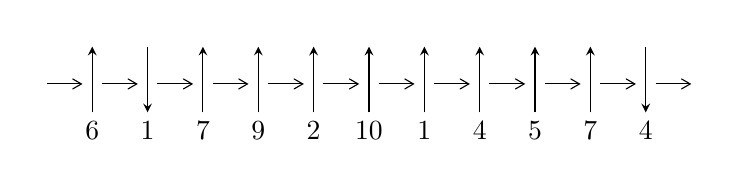
\begin{tikzpicture}[x=20pt, y=17pt]
	% nodes
	\node (C0) at (0, 0) {};
	\node (C1) at (1, 0) {};
	\node (C1U) at (1, +1) {};
	\node (C1D) at (1, -1) {6};

	\node (C2) at (2, 0) {};
	\node (C2U) at (2, +1) {};
	\node (C2D) at (2, -1) {1};

	\node (C3) at (3, 0) {};
	\node (C3U) at (3, +1) {};
	\node (C3D) at (3, -1) {7};

	\node (C4) at (4, 0) {};
	\node (C4U) at (4, +1) {};
	\node (C4D) at (4, -1) {9};

	\node (C5) at (5, 0) {};
	\node (C5U) at (5, +1) {};
	\node (C5D) at (5, -1) {2};

	\node (C6) at (6, 0) {};
	\node (C6U) at (6, +1) {};
	\node (C6D) at (6, -1) {10};

	\node (C7) at (7, 0) {};
	\node (C7U) at (7, +1) {};
	\node (C7D) at (7, -1) {1};

	\node (C8) at (8, 0) {};
	\node (C8U) at (8, +1) {};
	\node (C8D) at (8, -1) {4};

	\node (C9) at (9, 0) {};
	\node (C9U) at (9, +1) {};
	\node (C9D) at (9, -1) {5};

	\node (C10) at (10, 0) {};
	\node (C10U) at (10, +1) {};
	\node (C10D) at (10, -1) {7};

	\node (C11) at (11, 0) {};
	\node (C11U) at (11, +1) {};
	\node (C11D) at (11, -1) {4};
	\node (C12) at (12, 0) {};

	% arrows
	\draw[->,>={angle 60}]
	(C0) edge (C1) (C1) edge (C2) (C2) edge (C3) (C3) edge (C4) (C4) edge (C5) (C5) edge (C6) (C6) edge (C7) (C7) edge (C8) (C8) edge (C9) (C9) edge (C10) (C10) edge (C11) (C11) edge (C12) ;	\draw[->,>=stealth]
	(C1D) edge (C1U) (C2U) edge (C2D) (C3D) edge (C3U) (C4D) edge (C4U) (C5D) edge (C5U) (C6D) edge (C6U) (C7D) edge (C7U) (C8D) edge (C8U) (C9D) edge (C9U) (C10D) edge (C10U) (C11U) edge (C11D) ;
	\end{tikzpicture} \\
\hhline{~~} \\& 
\textbf{Solving Sequence} \\ \cline{2-2} 
 &
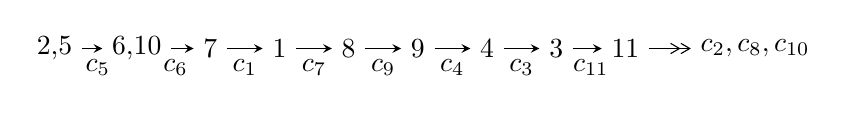
\begin{tikzpicture}[x=25pt, y=7pt]
	% node
	\node (A0) at (-1/8, 0) {2,5};
	\node (A1) at (17/16, 0) {6,10};
	\node (A2) at (17/8, 0) {7};
	\node (A3) at (25/8, 0) {1};
	\node (A4) at (33/8, 0) {8};
	\node (A5) at (41/8, 0) {9};
	\node (A6) at (49/8, 0) {4};
	\node (A7) at (57/8, 0) {3};
	\node (A8) at (65/8, 0) {11};
	\node (C1) at (1/2, -1) {$c_{5}$};
	\node (C2) at (13/8, -1) {$c_{6}$};
	\node (C3) at (21/8, -1) {$c_{1}$};
	\node (C4) at (29/8, -1) {$c_{7}$};
	\node (C5) at (37/8, -1) {$c_{9}$};
	\node (C6) at (45/8, -1) {$c_{4}$};
	\node (C7) at (53/8, -1) {$c_{3}$};
	\node (C8) at (61/8, -1) {$c_{11}$};
	\node (A9) at (10, 0) {$c_{2},c_{8},c_{10}$};

	% edge
	\draw[->,>=stealth]	
	(A0) edge (A1) (A1) edge (A2) (A2) edge (A3) (A3) edge (A4) (A4) edge (A5) (A5) edge (A6) (A6) edge (A7) (A7) edge (A8) ;
	\draw[->>,>={angle 60}]	
	(A8) edge (A9);
\end{tikzpicture} \\ 

\end{tabular} \\

\footnotetext{
The image of knot diagram is generated by the software ``\textbf{Draw programme}" developed by Andrew Bartholomew(\url{http://www.layer8.co.uk/maths/draw/index.htm\#Running-draw}), where we modified some parts for our purpose(\url{https://github.com/CATsTAILs/LinksPainter}).
}\phantom \\ \newline 
\centering \textbf{Ideals for irreducible components\footnotemark of $X_{\text{par}}$} 
 
\begin{align*}
I^u_{1}&=\langle 
3.53910\times10^{25} u^{37}-4.74008\times10^{25} u^{36}+\cdots+3.48267\times10^{25} b-4.36228\times10^{24},\\
\phantom{I^u_{1}}&\phantom{= \langle  }2.88601\times10^{25} u^{37}-3.57200\times10^{25} u^{36}+\cdots+3.48267\times10^{25} a+4.29759\times10^{24},\;u^{38}-2 u^{37}+\cdots-3 u+1\rangle \\
I^u_{2}&=\langle 
- u^9-3 u^7+u^6-4 u^5+2 u^4-3 u^3+u^2+b+1,\\
\phantom{I^u_{2}}&\phantom{= \langle  }u^9+3 u^8+6 u^7+10 u^6+12 u^5+14 u^4+12 u^3+12 u^2+a+8 u+4,\\
\phantom{I^u_{2}}&\phantom{= \langle  }u^{10}+u^9+4 u^8+3 u^7+7 u^6+4 u^5+7 u^4+4 u^3+4 u^2+u+1\rangle \\
\\
\end{align*}
\raggedright * 2 irreducible components of $\dim_{\mathbb{C}}=0$, with total 48 representations.\\
\footnotetext{All coefficients of polynomials are rational numbers. But the coefficients are sometimes approximated in decimal forms when there is not enough margin.}
\newpage
\renewcommand{\arraystretch}{1}
\centering \section*{I. $I^u_{1}= \langle 3.54\times10^{25} u^{37}-4.74\times10^{25} u^{36}+\cdots+3.48\times10^{25} b-4.36\times10^{24},\;2.89\times10^{25} u^{37}-3.57\times10^{25} u^{36}+\cdots+3.48\times10^{25} a+4.30\times10^{24},\;u^{38}-2 u^{37}+\cdots-3 u+1 \rangle$}
\flushleft \textbf{(i) Arc colorings}\\
\begin{tabular}{m{7pt} m{180pt} m{7pt} m{180pt} }
\flushright $a_{2}=$&$\begin{pmatrix}0\\u\end{pmatrix}$ \\
\flushright $a_{5}=$&$\begin{pmatrix}1\\0\end{pmatrix}$ \\
\flushright $a_{6}=$&$\begin{pmatrix}1\\- u^2\end{pmatrix}$ \\
\flushright $a_{10}=$&$\begin{pmatrix}-0.828678 u^{37}+1.02565 u^{36}+\cdots-2.81126 u-0.123399\\-1.01620 u^{37}+1.36105 u^{36}+\cdots-0.588254 u+0.125257\end{pmatrix}$ \\
\flushright $a_{7}=$&$\begin{pmatrix}0.631271 u^{37}+0.581742 u^{36}+\cdots-2.12748 u+3.40130\\-0.642147 u^{37}+1.04198 u^{36}+\cdots-0.717938 u+0.0244084\end{pmatrix}$ \\
\flushright $a_{1}=$&$\begin{pmatrix}- u\\u^3+u\end{pmatrix}$ \\
\flushright $a_{8}=$&$\begin{pmatrix}0.607524 u^{37}-0.145250 u^{36}+\cdots+0.310068 u+2.19514\\-0.307663 u^{37}+0.666840 u^{36}+\cdots-0.855780 u+0.456085\end{pmatrix}$ \\
\flushright $a_{9}=$&$\begin{pmatrix}0.187524 u^{37}-0.335397 u^{36}+\cdots-2.22301 u-0.248656\\-1.01620 u^{37}+1.36105 u^{36}+\cdots-0.588254 u+0.125257\end{pmatrix}$ \\
\flushright $a_{4}=$&$\begin{pmatrix}-1.27334 u^{37}+1.88196 u^{36}+\cdots+0.0209510 u-0.151656\\1.28508 u^{37}-2.98814 u^{36}+\cdots+3.97779 u-1.10711\end{pmatrix}$ \\
\flushright $a_{3}=$&$\begin{pmatrix}- u^3\\u^5+u^3+u\end{pmatrix}$ \\
\flushright $a_{11}=$&$\begin{pmatrix}-0.0155744 u^{37}+0.751097 u^{36}+\cdots-1.99782 u+0.341364\\-1.31911 u^{37}+1.47526 u^{36}+\cdots-3.17447 u+0.821375\end{pmatrix}$\\ \flushright $a_{11}=$&$\begin{pmatrix}-0.0155744 u^{37}+0.751097 u^{36}+\cdots-1.99782 u+0.341364\\-1.31911 u^{37}+1.47526 u^{36}+\cdots-3.17447 u+0.821375\end{pmatrix}$\\&\end{tabular}
\flushleft \textbf{(ii) Obstruction class $= -1$}\\~\\
\flushleft \textbf{(iii) Cusp Shapes $= -\frac{134839754017820031393971870}{34826691050833540478655473} u^{37}+\frac{3307262072424404195903844}{440844190516880259223487} u^{36}+\cdots-\frac{433267787549488445549936384}{34826691050833540478655473} u+\frac{614901013376164862123029830}{34826691050833540478655473}$}\\~\\
\newpage\renewcommand{\arraystretch}{1}
\flushleft \textbf{(iv) u-Polynomials at the component}\newline \\
\begin{tabular}{m{50pt}|m{274pt}}
Crossings & \hspace{64pt}u-Polynomials at each crossing \\
\hline $$\begin{aligned}c_{1},c_{5}\end{aligned}$$&$\begin{aligned}
&u^{38}-2 u^{37}+\cdots-3 u+1
\end{aligned}$\\
\hline $$\begin{aligned}c_{2}\end{aligned}$$&$\begin{aligned}
&u^{38}+20 u^{37}+\cdots-7 u+1
\end{aligned}$\\
\hline $$\begin{aligned}c_{3}\end{aligned}$$&$\begin{aligned}
&u^{38}- u^{37}+\cdots-130 u-29
\end{aligned}$\\
\hline $$\begin{aligned}c_{4},c_{8},c_{9}\end{aligned}$$&$\begin{aligned}
&u^{38}+u^{37}+\cdots-24 u-19
\end{aligned}$\\
\hline $$\begin{aligned}c_{6},c_{10}\end{aligned}$$&$\begin{aligned}
&u^{38}-3 u^{37}+\cdots+94 u-11
\end{aligned}$\\
\hline $$\begin{aligned}c_{7}\end{aligned}$$&$\begin{aligned}
&u^{38}+u^{37}+\cdots-39 u-2
\end{aligned}$\\
\hline $$\begin{aligned}c_{11}\end{aligned}$$&$\begin{aligned}
&u^{38}-2 u^{37}+\cdots+31 u+1
\end{aligned}$\\
\hline
\end{tabular}\\~\\
\newpage\renewcommand{\arraystretch}{1}
\flushleft \textbf{(v) Riley Polynomials at the component}\newline \\
\begin{tabular}{m{50pt}|m{274pt}}
Crossings & \hspace{64pt}Riley Polynomials at each crossing \\
\hline $$\begin{aligned}c_{1},c_{5}\end{aligned}$$&$\begin{aligned}
&y^{38}+20 y^{37}+\cdots-7 y+1
\end{aligned}$\\
\hline $$\begin{aligned}c_{2}\end{aligned}$$&$\begin{aligned}
&y^{38}+4 y^{37}+\cdots-95 y+1
\end{aligned}$\\
\hline $$\begin{aligned}c_{3}\end{aligned}$$&$\begin{aligned}
&y^{38}+41 y^{37}+\cdots+1138 y+841
\end{aligned}$\\
\hline $$\begin{aligned}c_{4},c_{8},c_{9}\end{aligned}$$&$\begin{aligned}
&y^{38}-35 y^{37}+\cdots-6 y+361
\end{aligned}$\\
\hline $$\begin{aligned}c_{6},c_{10}\end{aligned}$$&$\begin{aligned}
&y^{38}-17 y^{37}+\cdots-1686 y+121
\end{aligned}$\\
\hline $$\begin{aligned}c_{7}\end{aligned}$$&$\begin{aligned}
&y^{38}+37 y^{37}+\cdots-325 y+4
\end{aligned}$\\
\hline $$\begin{aligned}c_{11}\end{aligned}$$&$\begin{aligned}
&y^{38}-38 y^{37}+\cdots-415 y+1
\end{aligned}$\\
\hline
\end{tabular}\\~\\
\newpage\flushleft \textbf{(vi) Complex Volumes and Cusp Shapes}
$$\begin{array}{c|c|c}  
\text{Solutions to }I^u_{1}& \I (\text{vol} + \sqrt{-1}CS) & \text{Cusp shape}\\
 \hline 
\begin{aligned}
u &= \phantom{-}0.198690 + 0.927706 I \\
a &= -0.29365 - 1.42984 I \\
b &= -0.507231 - 0.501686 I\end{aligned}
 & -1.65932 + 1.72508 I & \phantom{-}3.99615 - 5.00557 I \\ \hline\begin{aligned}
u &= \phantom{-}0.198690 - 0.927706 I \\
a &= -0.29365 + 1.42984 I \\
b &= -0.507231 + 0.501686 I\end{aligned}
 & -1.65932 - 1.72508 I & \phantom{-}3.99615 + 5.00557 I \\ \hline\begin{aligned}
u &= -0.379743 + 0.859856 I \\
a &= -0.035838 + 1.400050 I \\
b &= \phantom{-}0.285476 + 0.554000 I\end{aligned}
 & \phantom{-}1.30138 - 1.64549 I & \phantom{-}4.54049 - 1.93386 I \\ \hline\begin{aligned}
u &= -0.379743 - 0.859856 I \\
a &= -0.035838 - 1.400050 I \\
b &= \phantom{-}0.285476 - 0.554000 I\end{aligned}
 & \phantom{-}1.30138 + 1.64549 I & \phantom{-}4.54049 + 1.93386 I \\ \hline\begin{aligned}
u &= \phantom{-}0.437061 + 1.002290 I \\
a &= \phantom{-}0.802004 - 0.659495 I \\
b &= \phantom{-}1.178350 - 0.751371 I\end{aligned}
 & -3.43318 + 1.20443 I & \phantom{-}6.92259 - 2.66519 I \\ \hline\begin{aligned}
u &= \phantom{-}0.437061 - 1.002290 I \\
a &= \phantom{-}0.802004 + 0.659495 I \\
b &= \phantom{-}1.178350 + 0.751371 I\end{aligned}
 & -3.43318 - 1.20443 I & \phantom{-}6.92259 + 2.66519 I \\ \hline\begin{aligned}
u &= \phantom{-}0.668607 + 0.872893 I \\
a &= -0.468782 + 0.686829 I \\
b &= -0.086247 + 0.537690 I\end{aligned}
 & \phantom{-}1.01360 + 2.58424 I & \phantom{-}2.68887 - 3.99949 I \\ \hline\begin{aligned}
u &= \phantom{-}0.668607 - 0.872893 I \\
a &= -0.468782 - 0.686829 I \\
b &= -0.086247 - 0.537690 I\end{aligned}
 & \phantom{-}1.01360 - 2.58424 I & \phantom{-}2.68887 + 3.99949 I \\ \hline\begin{aligned}
u &= \phantom{-}0.496586 + 1.000340 I \\
a &= -0.81802 + 1.31551 I \\
b &= \phantom{-}1.39385 + 0.31403 I\end{aligned}
 & -3.05076 + 4.70281 I & \phantom{-}7.22690 - 4.71362 I \\ \hline\begin{aligned}
u &= \phantom{-}0.496586 - 1.000340 I \\
a &= -0.81802 - 1.31551 I \\
b &= \phantom{-}1.39385 - 0.31403 I\end{aligned}
 & -3.05076 - 4.70281 I & \phantom{-}7.22690 + 4.71362 I\\
 \hline 
 \end{array}$$\newpage$$\begin{array}{c|c|c}  
\text{Solutions to }I^u_{1}& \I (\text{vol} + \sqrt{-1}CS) & \text{Cusp shape}\\
 \hline 
\begin{aligned}
u &= \phantom{-}1.081330 + 0.386328 I \\
a &= -0.216812 - 0.071474 I \\
b &= \phantom{-}1.43091 - 0.33793 I\end{aligned}
 & \phantom{-}1.95602 - 6.72677 I & \phantom{-}10.60803 + 3.77299 I \\ \hline\begin{aligned}
u &= \phantom{-}1.081330 - 0.386328 I \\
a &= -0.216812 + 0.071474 I \\
b &= \phantom{-}1.43091 + 0.33793 I\end{aligned}
 & \phantom{-}1.95602 + 6.72677 I & \phantom{-}10.60803 - 3.77299 I \\ \hline\begin{aligned}
u &= -0.775393 + 0.236076 I \\
a &= -0.744379 - 0.266250 I \\
b &= -0.299152 - 0.795595 I\end{aligned}
 & -3.53482 + 2.58667 I & \phantom{-}7.16756 - 2.58418 I \\ \hline\begin{aligned}
u &= -0.775393 - 0.236076 I \\
a &= -0.744379 + 0.266250 I \\
b &= -0.299152 + 0.795595 I\end{aligned}
 & -3.53482 - 2.58667 I & \phantom{-}7.16756 + 2.58418 I \\ \hline\begin{aligned}
u &= -0.913408 + 0.776527 I \\
a &= -0.296533 - 0.156951 I \\
b &= \phantom{-}1.287170 + 0.114756 I\end{aligned}
 & \phantom{-}5.31271 - 0.53174 I & \phantom{-}10.57597 + 0.24868 I \\ \hline\begin{aligned}
u &= -0.913408 - 0.776527 I \\
a &= -0.296533 + 0.156951 I \\
b &= \phantom{-}1.287170 - 0.114756 I\end{aligned}
 & \phantom{-}5.31271 + 0.53174 I & \phantom{-}10.57597 - 0.24868 I \\ \hline\begin{aligned}
u &= \phantom{-}0.447680 + 0.663750 I \\
a &= \phantom{-}0.97208 - 2.47509 I \\
b &= -1.110300 + 0.132355 I\end{aligned}
 & -1.90577 - 0.72497 I & \phantom{-}8.59505 - 1.33995 I \\ \hline\begin{aligned}
u &= \phantom{-}0.447680 - 0.663750 I \\
a &= \phantom{-}0.97208 + 2.47509 I \\
b &= -1.110300 - 0.132355 I\end{aligned}
 & -1.90577 + 0.72497 I & \phantom{-}8.59505 + 1.33995 I \\ \hline\begin{aligned}
u &= -0.526939 + 1.137220 I \\
a &= \phantom{-}0.54259 - 1.42286 I \\
b &= \phantom{-}1.53921 - 0.16530 I\end{aligned}
 & \phantom{-}5.23331 - 4.18634 I & \phantom{-}5.68349 + 3.29449 I \\ \hline\begin{aligned}
u &= -0.526939 - 1.137220 I \\
a &= \phantom{-}0.54259 + 1.42286 I \\
b &= \phantom{-}1.53921 + 0.16530 I\end{aligned}
 & \phantom{-}5.23331 + 4.18634 I & \phantom{-}5.68349 - 3.29449 I\\
 \hline 
 \end{array}$$\newpage$$\begin{array}{c|c|c}  
\text{Solutions to }I^u_{1}& \I (\text{vol} + \sqrt{-1}CS) & \text{Cusp shape}\\
 \hline 
\begin{aligned}
u &= -0.784887 + 0.992111 I \\
a &= \phantom{-}0.32772 + 1.44641 I \\
b &= -1.252110 + 0.274462 I\end{aligned}
 & \phantom{-}4.61276 - 5.70694 I & \phantom{-}9.04865 + 6.07255 I \\ \hline\begin{aligned}
u &= -0.784887 - 0.992111 I \\
a &= \phantom{-}0.32772 - 1.44641 I \\
b &= -1.252110 - 0.274462 I\end{aligned}
 & \phantom{-}4.61276 + 5.70694 I & \phantom{-}9.04865 - 6.07255 I \\ \hline\begin{aligned}
u &= -0.561660 + 1.148650 I \\
a &= -0.34487 - 1.38992 I \\
b &= \phantom{-}0.258106 - 1.087690 I\end{aligned}
 & -6.14363 - 7.57123 I & \phantom{-}4.89087 + 5.76194 I \\ \hline\begin{aligned}
u &= -0.561660 - 1.148650 I \\
a &= -0.34487 + 1.38992 I \\
b &= \phantom{-}0.258106 + 1.087690 I\end{aligned}
 & -6.14363 + 7.57123 I & \phantom{-}4.89087 - 5.76194 I \\ \hline\begin{aligned}
u &= -0.297248 + 1.257890 I \\
a &= \phantom{-}0.693796 + 0.789863 I \\
b &= -0.164859 + 0.672738 I\end{aligned}
 & -8.06788 - 1.04561 I & \phantom{-}1.73854 + 0.76531 I \\ \hline\begin{aligned}
u &= -0.297248 - 1.257890 I \\
a &= \phantom{-}0.693796 - 0.789863 I \\
b &= -0.164859 - 0.672738 I\end{aligned}
 & -8.06788 + 1.04561 I & \phantom{-}1.73854 - 0.76531 I \\ \hline\begin{aligned}
u &= \phantom{-}0.693371\phantom{ +0.000000I} \\
a &= -0.324535\phantom{ +0.000000I} \\
b &= -1.38702\phantom{ +0.000000I}\end{aligned}
 & \phantom{-}7.32047\phantom{ +0.000000I} & \phantom{-}11.7760\phantom{ +0.000000I} \\ \hline\begin{aligned}
u &= \phantom{-}0.534109 + 1.201300 I \\
a &= \phantom{-}0.76686 + 1.35110 I \\
b &= \phantom{-}1.196420 + 0.245037 I\end{aligned}
 & \phantom{-}4.11680 + 4.64818 I & \phantom{-}7.00000 - 4.11714 I \\ \hline\begin{aligned}
u &= \phantom{-}0.534109 - 1.201300 I \\
a &= \phantom{-}0.76686 - 1.35110 I \\
b &= \phantom{-}1.196420 - 0.245037 I\end{aligned}
 & \phantom{-}4.11680 - 4.64818 I & \phantom{-}7.00000 + 4.11714 I \\ \hline\begin{aligned}
u &= \phantom{-}0.326007 + 0.583311 I \\
a &= -0.52323 - 2.59696 I \\
b &= -0.878482 - 0.628167 I\end{aligned}
 & -2.08165 + 2.22554 I & \phantom{-}9.62442 - 6.36612 I\\
 \hline 
 \end{array}$$\newpage$$\begin{array}{c|c|c}  
\text{Solutions to }I^u_{1}& \I (\text{vol} + \sqrt{-1}CS) & \text{Cusp shape}\\
 \hline 
\begin{aligned}
u &= \phantom{-}0.326007 - 0.583311 I \\
a &= -0.52323 + 2.59696 I \\
b &= -0.878482 + 0.628167 I\end{aligned}
 & -2.08165 - 2.22554 I & \phantom{-}9.62442 + 6.36612 I \\ \hline\begin{aligned}
u &= \phantom{-}0.698047 + 1.223380 I \\
a &= -0.14107 - 1.57898 I \\
b &= -1.47736 - 0.45823 I\end{aligned}
 & -0.64182 + 13.08690 I & \phantom{-0.000000 } 0 \\ \hline\begin{aligned}
u &= \phantom{-}0.698047 - 1.223380 I \\
a &= -0.14107 + 1.57898 I \\
b &= -1.47736 + 0.45823 I\end{aligned}
 & -0.64182 - 13.08690 I & \phantom{-0.000000 } 0 \\ \hline\begin{aligned}
u &= \phantom{-}0.19948 + 1.53203 I \\
a &= -0.874606 + 0.019930 I \\
b &= -1.233390 + 0.241654 I\end{aligned}
 & -4.80130 - 2.15880 I & \phantom{-0.000000 } 0 \\ \hline\begin{aligned}
u &= \phantom{-}0.19948 - 1.53203 I \\
a &= -0.874606 - 0.019930 I \\
b &= -1.233390 - 0.241654 I\end{aligned}
 & -4.80130 + 2.15880 I & \phantom{-0.000000 } 0 \\ \hline\begin{aligned}
u &= -0.337441 + 0.249883 I \\
a &= \phantom{-}1.16350 + 0.97340 I \\
b &= -1.59455 + 0.00504 I\end{aligned}
 & \phantom{-}7.79085 - 0.03851 I & \phantom{-}8.05729 - 1.80582 I \\ \hline\begin{aligned}
u &= -0.337441 - 0.249883 I \\
a &= \phantom{-}1.16350 - 0.97340 I \\
b &= -1.59455 - 0.00504 I\end{aligned}
 & \phantom{-}7.79085 + 0.03851 I & \phantom{-}8.05729 + 1.80582 I \\ \hline\begin{aligned}
u &= \phantom{-}0.284870\phantom{ +0.000000I} \\
a &= -0.696967\phantom{ +0.000000I} \\
b &= \phantom{-}0.455407\phantom{ +0.000000I}\end{aligned}
 & \phantom{-}0.644934\phantom{ +0.000000I} & \phantom{-}15.5790\phantom{ +0.000000I}\\
 \hline 
 \end{array}$$\newpage\newpage\renewcommand{\arraystretch}{1}
\centering \section*{II. $I^u_{2}= \langle - u^9-3 u^7+\cdots+b+1,\;u^9+3 u^8+\cdots+a+4,\;u^{10}+u^9+\cdots+u+1 \rangle$}
\flushleft \textbf{(i) Arc colorings}\\
\begin{tabular}{m{7pt} m{180pt} m{7pt} m{180pt} }
\flushright $a_{2}=$&$\begin{pmatrix}0\\u\end{pmatrix}$ \\
\flushright $a_{5}=$&$\begin{pmatrix}1\\0\end{pmatrix}$ \\
\flushright $a_{6}=$&$\begin{pmatrix}1\\- u^2\end{pmatrix}$ \\
\flushright $a_{10}=$&$\begin{pmatrix}- u^9-3 u^8-6 u^7-10 u^6-12 u^5-14 u^4-12 u^3-12 u^2-8 u-4\\u^9+3 u^7- u^6+4 u^5-2 u^4+3 u^3- u^2-1\end{pmatrix}$ \\
\flushright $a_{7}=$&$\begin{pmatrix}2 u^9+u^8+6 u^7+u^6+8 u^5- u^4+6 u^3+u-2\\u^8+3 u^6+4 u^4+2 u^2+u\end{pmatrix}$ \\
\flushright $a_{1}=$&$\begin{pmatrix}- u\\u^3+u\end{pmatrix}$ \\
\flushright $a_{8}=$&$\begin{pmatrix}u^9+3 u^7- u^6+4 u^5-3 u^4+3 u^3-2 u^2-2\\u^8+3 u^6+4 u^4+3 u^2+u\end{pmatrix}$ \\
\flushright $a_{9}=$&$\begin{pmatrix}-2 u^9-3 u^8-9 u^7-9 u^6-16 u^5-12 u^4-15 u^3-11 u^2-8 u-3\\u^9+3 u^7- u^6+4 u^5-2 u^4+3 u^3- u^2-1\end{pmatrix}$ \\
\flushright $a_{4}=$&$\begin{pmatrix}u^9+3 u^8+5 u^7+9 u^6+9 u^5+12 u^4+8 u^3+10 u^2+6 u+2\\u^9+u^8+4 u^7+3 u^6+7 u^5+4 u^4+7 u^3+4 u^2+3 u+2\end{pmatrix}$ \\
\flushright $a_{3}=$&$\begin{pmatrix}- u^3\\u^5+u^3+u\end{pmatrix}$ \\
\flushright $a_{11}=$&$\begin{pmatrix}-2 u^9-5 u^8-10 u^7-16 u^6-18 u^5-22 u^4-17 u^3-19 u^2-12 u-5\\- u^7- u^6-3 u^5-2 u^4-3 u^3-2 u^2-2 u-2\end{pmatrix}$\\ \flushright $a_{11}=$&$\begin{pmatrix}-2 u^9-5 u^8-10 u^7-16 u^6-18 u^5-22 u^4-17 u^3-19 u^2-12 u-5\\- u^7- u^6-3 u^5-2 u^4-3 u^3-2 u^2-2 u-2\end{pmatrix}$\\&\end{tabular}
\flushleft \textbf{(ii) Obstruction class $= 1$}\\~\\
\flushleft \textbf{(iii) Cusp Shapes $= 6 u^9+u^8+19 u^7- u^6+26 u^5-10 u^4+20 u^3-9 u^2+2 u$}\\~\\
\newpage\renewcommand{\arraystretch}{1}
\flushleft \textbf{(iv) u-Polynomials at the component}\newline \\
\begin{tabular}{m{50pt}|m{274pt}}
Crossings & \hspace{64pt}u-Polynomials at each crossing \\
\hline $$\begin{aligned}c_{1}\end{aligned}$$&$\begin{aligned}
&u^{10}- u^9+4 u^8-3 u^7+7 u^6-4 u^5+7 u^4-4 u^3+4 u^2- u+1
\end{aligned}$\\
\hline $$\begin{aligned}c_{2}\end{aligned}$$&$\begin{aligned}
&u^{10}+7 u^9+\cdots+7 u+1
\end{aligned}$\\
\hline $$\begin{aligned}c_{3}\end{aligned}$$&$\begin{aligned}
&u^{10}+2 u^8+u^7-4 u^6-2 u^5-2 u^4-2 u^3+8 u^2-2 u+1
\end{aligned}$\\
\hline $$\begin{aligned}c_{4}\end{aligned}$$&$\begin{aligned}
&u^{10}-6 u^8- u^7+13 u^6+4 u^5-12 u^4-5 u^3+4 u^2+2 u+1
\end{aligned}$\\
\hline $$\begin{aligned}c_{5}\end{aligned}$$&$\begin{aligned}
&u^{10}+u^9+4 u^8+3 u^7+7 u^6+4 u^5+7 u^4+4 u^3+4 u^2+u+1
\end{aligned}$\\
\hline $$\begin{aligned}c_{6}\end{aligned}$$&$\begin{aligned}
&u^{10}-2 u^9- u^8+3 u^7+u^5-2 u^4-2 u^3+2 u^2+1
\end{aligned}$\\
\hline $$\begin{aligned}c_{7}\end{aligned}$$&$\begin{aligned}
&u^{10}+2 u^8-2 u^7-2 u^6+u^5+3 u^3- u^2-2 u+1
\end{aligned}$\\
\hline $$\begin{aligned}c_{8},c_{9}\end{aligned}$$&$\begin{aligned}
&u^{10}-6 u^8+u^7+13 u^6-4 u^5-12 u^4+5 u^3+4 u^2-2 u+1
\end{aligned}$\\
\hline $$\begin{aligned}c_{10}\end{aligned}$$&$\begin{aligned}
&u^{10}+2 u^9- u^8-3 u^7- u^5-2 u^4+2 u^3+2 u^2+1
\end{aligned}$\\
\hline $$\begin{aligned}c_{11}\end{aligned}$$&$\begin{aligned}
&u^{10}-3 u^9+u^8+5 u^7-7 u^6+3 u^5+4 u^4-7 u^3+6 u^2-3 u+1
\end{aligned}$\\
\hline
\end{tabular}\\~\\
\newpage\renewcommand{\arraystretch}{1}
\flushleft \textbf{(v) Riley Polynomials at the component}\newline \\
\begin{tabular}{m{50pt}|m{274pt}}
Crossings & \hspace{64pt}Riley Polynomials at each crossing \\
\hline $$\begin{aligned}c_{1},c_{5}\end{aligned}$$&$\begin{aligned}
&y^{10}+7 y^9+\cdots+7 y+1
\end{aligned}$\\
\hline $$\begin{aligned}c_{2}\end{aligned}$$&$\begin{aligned}
&y^{10}- y^9+\cdots-5 y+1
\end{aligned}$\\
\hline $$\begin{aligned}c_{3}\end{aligned}$$&$\begin{aligned}
&y^{10}+4 y^9+\cdots+12 y+1
\end{aligned}$\\
\hline $$\begin{aligned}c_{4},c_{8},c_{9}\end{aligned}$$&$\begin{aligned}
&y^{10}-12 y^9+\cdots+4 y+1
\end{aligned}$\\
\hline $$\begin{aligned}c_{6},c_{10}\end{aligned}$$&$\begin{aligned}
&y^{10}-6 y^9+13 y^8-9 y^7-6 y^6+9 y^5+6 y^4-12 y^3+4 y+1
\end{aligned}$\\
\hline $$\begin{aligned}c_{7}\end{aligned}$$&$\begin{aligned}
&y^{10}+4 y^9-12 y^7+6 y^6+9 y^5-6 y^4-9 y^3+13 y^2-6 y+1
\end{aligned}$\\
\hline $$\begin{aligned}c_{11}\end{aligned}$$&$\begin{aligned}
&y^{10}-7 y^9+17 y^8-13 y^7-3 y^6+y^5+6 y^4+3 y^3+2 y^2+3 y+1
\end{aligned}$\\
\hline
\end{tabular}\\~\\
\newpage\flushleft \textbf{(vi) Complex Volumes and Cusp Shapes}
$$\begin{array}{c|c|c}  
\text{Solutions to }I^u_{2}& \I (\text{vol} + \sqrt{-1}CS) & \text{Cusp shape}\\
 \hline 
\begin{aligned}
u &= \phantom{-}0.591573 + 0.895458 I \\
a &= -0.062941 + 0.916484 I \\
b &= -0.162645 + 0.362811 I\end{aligned}
 & \phantom{-}1.88316 + 2.32533 I & \phantom{-}12.32535 - 3.44072 I \\ \hline\begin{aligned}
u &= \phantom{-}0.591573 - 0.895458 I \\
a &= -0.062941 - 0.916484 I \\
b &= -0.162645 - 0.362811 I\end{aligned}
 & \phantom{-}1.88316 - 2.32533 I & \phantom{-}12.32535 + 3.44072 I \\ \hline\begin{aligned}
u &= -0.587969 + 0.580983 I \\
a &= -0.270490 - 0.170382 I \\
b &= \phantom{-}1.56713 + 0.08593 I\end{aligned}
 & \phantom{-}8.26505 - 0.63915 I & \phantom{-}14.5970 + 5.3987 I \\ \hline\begin{aligned}
u &= -0.587969 - 0.580983 I \\
a &= -0.270490 + 0.170382 I \\
b &= \phantom{-}1.56713 - 0.08593 I\end{aligned}
 & \phantom{-}8.26505 + 0.63915 I & \phantom{-}14.5970 - 5.3987 I \\ \hline\begin{aligned}
u &= -0.642090 + 1.139230 I \\
a &= -0.42175 + 1.41771 I \\
b &= -1.43000 + 0.16541 I\end{aligned}
 & \phantom{-}6.43677 - 4.34705 I & \phantom{-}13.62063 + 3.59101 I \\ \hline\begin{aligned}
u &= -0.642090 - 1.139230 I \\
a &= -0.42175 - 1.41771 I \\
b &= -1.43000 - 0.16541 I\end{aligned}
 & \phantom{-}6.43677 + 4.34705 I & \phantom{-}13.62063 - 3.59101 I \\ \hline\begin{aligned}
u &= \phantom{-}0.059179 + 1.329340 I \\
a &= \phantom{-}0.597845 + 0.216685 I \\
b &= \phantom{-}0.995882 - 0.290486 I\end{aligned}
 & -5.58838 - 1.13850 I & \phantom{-}4.94587 - 0.33361 I \\ \hline\begin{aligned}
u &= \phantom{-}0.059179 - 1.329340 I \\
a &= \phantom{-}0.597845 - 0.216685 I \\
b &= \phantom{-}0.995882 + 0.290486 I\end{aligned}
 & -5.58838 + 1.13850 I & \phantom{-}4.94587 + 0.33361 I \\ \hline\begin{aligned}
u &= \phantom{-}0.079307 + 0.642927 I \\
a &= -0.84267 - 3.52089 I \\
b &= -0.970365 - 0.458151 I\end{aligned}
 & -2.77192 + 1.74853 I & \phantom{-}1.51113 - 2.06464 I \\ \hline\begin{aligned}
u &= \phantom{-}0.079307 - 0.642927 I \\
a &= -0.84267 + 3.52089 I \\
b &= -0.970365 + 0.458151 I\end{aligned}
 & -2.77192 - 1.74853 I & \phantom{-}1.51113 + 2.06464 I\\
 \hline 
 \end{array}$$\newpage
\newpage\renewcommand{\arraystretch}{1}
\centering \section*{ III. u-Polynomials}
\begin{tabular}{m{50pt}|m{274pt}}
Crossings & \hspace{64pt}u-Polynomials at each crossing \\
\hline $$\begin{aligned}c_{1}\end{aligned}$$&$\begin{aligned}
&(u^{10}- u^9+4 u^8-3 u^7+7 u^6-4 u^5+7 u^4-4 u^3+4 u^2- u+1)\\
&\cdot(u^{38}-2 u^{37}+\cdots-3 u+1)
\end{aligned}$\\
\hline $$\begin{aligned}c_{2}\end{aligned}$$&$\begin{aligned}
&(u^{10}+7 u^9+\cdots+7 u+1)(u^{38}+20 u^{37}+\cdots-7 u+1)
\end{aligned}$\\
\hline $$\begin{aligned}c_{3}\end{aligned}$$&$\begin{aligned}
&(u^{10}+2 u^8+u^7-4 u^6-2 u^5-2 u^4-2 u^3+8 u^2-2 u+1)\\
&\cdot(u^{38}- u^{37}+\cdots-130 u-29)
\end{aligned}$\\
\hline $$\begin{aligned}c_{4}\end{aligned}$$&$\begin{aligned}
&(u^{10}-6 u^8- u^7+13 u^6+4 u^5-12 u^4-5 u^3+4 u^2+2 u+1)\\
&\cdot(u^{38}+u^{37}+\cdots-24 u-19)
\end{aligned}$\\
\hline $$\begin{aligned}c_{5}\end{aligned}$$&$\begin{aligned}
&(u^{10}+u^9+4 u^8+3 u^7+7 u^6+4 u^5+7 u^4+4 u^3+4 u^2+u+1)\\
&\cdot(u^{38}-2 u^{37}+\cdots-3 u+1)
\end{aligned}$\\
\hline $$\begin{aligned}c_{6}\end{aligned}$$&$\begin{aligned}
&(u^{10}-2 u^9- u^8+3 u^7+u^5-2 u^4-2 u^3+2 u^2+1)\\
&\cdot(u^{38}-3 u^{37}+\cdots+94 u-11)
\end{aligned}$\\
\hline $$\begin{aligned}c_{7}\end{aligned}$$&$\begin{aligned}
&(u^{10}+2 u^8-2 u^7-2 u^6+u^5+3 u^3- u^2-2 u+1)\\
&\cdot(u^{38}+u^{37}+\cdots-39 u-2)
\end{aligned}$\\
\hline $$\begin{aligned}c_{8},c_{9}\end{aligned}$$&$\begin{aligned}
&(u^{10}-6 u^8+u^7+13 u^6-4 u^5-12 u^4+5 u^3+4 u^2-2 u+1)\\
&\cdot(u^{38}+u^{37}+\cdots-24 u-19)
\end{aligned}$\\
\hline $$\begin{aligned}c_{10}\end{aligned}$$&$\begin{aligned}
&(u^{10}+2 u^9- u^8-3 u^7- u^5-2 u^4+2 u^3+2 u^2+1)\\
&\cdot(u^{38}-3 u^{37}+\cdots+94 u-11)
\end{aligned}$\\
\hline $$\begin{aligned}c_{11}\end{aligned}$$&$\begin{aligned}
&(u^{10}-3 u^9+u^8+5 u^7-7 u^6+3 u^5+4 u^4-7 u^3+6 u^2-3 u+1)\\
&\cdot(u^{38}-2 u^{37}+\cdots+31 u+1)
\end{aligned}$\\
\hline
\end{tabular}\newpage\renewcommand{\arraystretch}{1}
\centering \section*{ IV. Riley Polynomials}
\begin{tabular}{m{50pt}|m{274pt}}
Crossings & \hspace{64pt}Riley Polynomials at each crossing \\
\hline $$\begin{aligned}c_{1},c_{5}\end{aligned}$$&$\begin{aligned}
&(y^{10}+7 y^9+\cdots+7 y+1)(y^{38}+20 y^{37}+\cdots-7 y+1)
\end{aligned}$\\
\hline $$\begin{aligned}c_{2}\end{aligned}$$&$\begin{aligned}
&(y^{10}- y^9+\cdots-5 y+1)(y^{38}+4 y^{37}+\cdots-95 y+1)
\end{aligned}$\\
\hline $$\begin{aligned}c_{3}\end{aligned}$$&$\begin{aligned}
&(y^{10}+4 y^9+\cdots+12 y+1)(y^{38}+41 y^{37}+\cdots+1138 y+841)
\end{aligned}$\\
\hline $$\begin{aligned}c_{4},c_{8},c_{9}\end{aligned}$$&$\begin{aligned}
&(y^{10}-12 y^9+\cdots+4 y+1)(y^{38}-35 y^{37}+\cdots-6 y+361)
\end{aligned}$\\
\hline $$\begin{aligned}c_{6},c_{10}\end{aligned}$$&$\begin{aligned}
&(y^{10}-6 y^9+13 y^8-9 y^7-6 y^6+9 y^5+6 y^4-12 y^3+4 y+1)\\
&\cdot(y^{38}-17 y^{37}+\cdots-1686 y+121)
\end{aligned}$\\
\hline $$\begin{aligned}c_{7}\end{aligned}$$&$\begin{aligned}
&(y^{10}+4 y^9-12 y^7+6 y^6+9 y^5-6 y^4-9 y^3+13 y^2-6 y+1)\\
&\cdot(y^{38}+37 y^{37}+\cdots-325 y+4)
\end{aligned}$\\
\hline $$\begin{aligned}c_{11}\end{aligned}$$&$\begin{aligned}
&(y^{10}-7 y^9+17 y^8-13 y^7-3 y^6+y^5+6 y^4+3 y^3+2 y^2+3 y+1)\\
&\cdot(y^{38}-38 y^{37}+\cdots-415 y+1)
\end{aligned}$\\
\hline
\end{tabular}
\vskip 2pc
\end{document}